\documentclass[tikz,border=2pt]{standalone}
\usepackage{amsmath,amssymb}
\usepackage{pgfplots}
\pgfplotsset{compat=1.18}
\usetikzlibrary{calc}

\begin{document}
% Skewness: which way the long tail points (right-skewed > 0, left-skewed < 0).
% Kurtosis: how heavy the tails are compared with the normal (excess kurtosis 0).
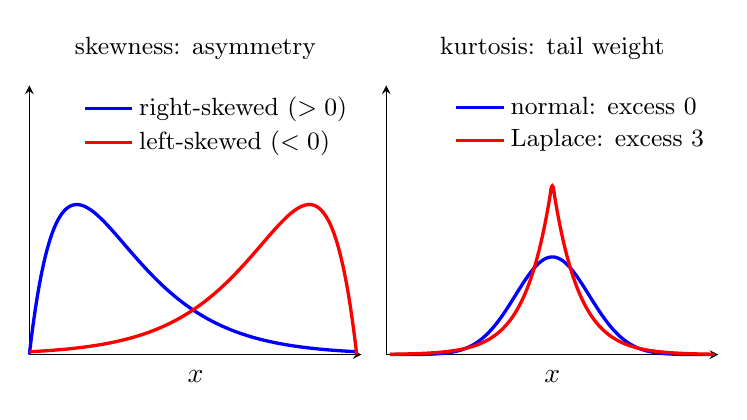
\begin{tikzpicture}
	\begin{axis}[
		name=p1, axis lines=left, xmin=0, xmax=7, ymin=0, ymax=0.66,
		xtick=\empty, ytick=\empty, xlabel={$x$},
		samples=160, smooth, width=5.8cm, height=5cm, clip=false, title={skewness: asymmetry}, title style={font=\small},
		legend style={draw=none, fill=none, font=\small, at={(1.0,1.0)}, anchor=north east}, legend cell align=left
		]
		\addplot[blue, very thick, domain=0:6.9] {x*exp(-x)};
		\addlegendentry{right-skewed ($>0$)}
		\addplot[red, very thick, domain=0:6.9] {(6.9-x)*exp(-(6.9-x))};
		\addlegendentry{left-skewed ($<0$)}
	\end{axis}
	\begin{axis}[
		name=p2, at={(p1.outer east)}, anchor=outer west, xshift=3mm,
		axis lines=left, xmin=-4.5, xmax=4.5, ymin=0, ymax=1.1,
		xtick=\empty, ytick=\empty, xlabel={$x$},
		samples=200, smooth, width=5.8cm, height=5cm, clip=false, title={kurtosis: tail weight}, title style={font=\small},
		legend style={draw=none, fill=none, font=\small, at={(1.0,1.0)}, anchor=north east}, legend cell align=left
		]
		\addplot[blue, very thick, domain=-4.4:4.4] {exp(-x^2/2)/sqrt(2*pi)};
		\addlegendentry{normal: excess $0$}
		\addplot[red, very thick, domain=-4.4:4.4] {exp(-abs(x)*sqrt(2))/sqrt(2)};
		\addlegendentry{Laplace: excess $3$}
	\end{axis}
	
\end{tikzpicture}
\end{document}
